
\documentclass[12pt]{article}
\usepackage{amsmath}
\usepackage{latexsym}
\usepackage{amsfonts}
\usepackage[normalem]{ulem}
\usepackage{array}
\usepackage{amssymb}
\usepackage{graphicx}
\usepackage[backend=biber,
style=numeric,
sorting=none,
isbn=false,
doi=false,
url=false,
]{biblatex}\addbibresource{bibliography.bib}

\usepackage{subfig}
\usepackage{wrapfig}
\usepackage{wasysym}
\usepackage{enumitem}
\usepackage{adjustbox}
\usepackage{ragged2e}
\usepackage[svgnames,table]{xcolor}
\usepackage{tikz}
\usepackage{longtable}
\usepackage{changepage}
\usepackage{setspace}
\usepackage{hhline}
\usepackage{multicol}
\usepackage{tabto}
\usepackage{float}
\usepackage{multirow}
\usepackage{makecell}
\usepackage{fancyhdr}
\usepackage[toc,page]{appendix}
\usepackage[hidelinks]{hyperref}
\usetikzlibrary{shapes.symbols,shapes.geometric,shadows,arrows.meta}
\tikzset{>={Latex[width=1.5mm,length=2mm]}}
\usepackage{flowchart}\usepackage[paperheight=11.0in,paperwidth=8.5in,left=0.5in,right=0.5in,top=0.5in,bottom=0.5in,headheight=1in]{geometry}
\usepackage[utf8]{inputenc}
\usepackage[T1]{fontenc}
\TabPositions{0.49in,0.98in,1.47in,1.96in,2.45in,2.94in,3.43in,3.92in,4.41in,4.9in,5.39in,5.88in,6.37in,6.86in,7.35in,}

\urlstyle{same}


 %%%%%%%%%%%%  Set Depths for Sections  %%%%%%%%%%%%%%

% 1) Section
% 1.1) SubSection
% 1.1.1) SubSubSection
% 1.1.1.1) Paragraph
% 1.1.1.1.1) Subparagraph


\setcounter{tocdepth}{5}
\setcounter{secnumdepth}{5}


 %%%%%%%%%%%%  Set Depths for Nested Lists created by \begin{enumerate}  %%%%%%%%%%%%%%


\setlistdepth{9}
\renewlist{enumerate}{enumerate}{9}
		\setlist[enumerate,1]{label=\arabic*)}
		\setlist[enumerate,2]{label=\alph*)}
		\setlist[enumerate,3]{label=(\roman*)}
		\setlist[enumerate,4]{label=(\arabic*)}
		\setlist[enumerate,5]{label=(\Alph*)}
		\setlist[enumerate,6]{label=(\Roman*)}
		\setlist[enumerate,7]{label=\arabic*}
		\setlist[enumerate,8]{label=\alph*}
		\setlist[enumerate,9]{label=\roman*}

\renewlist{itemize}{itemize}{9}
		\setlist[itemize]{label=$\cdot$}
		\setlist[itemize,1]{label=\textbullet}
		\setlist[itemize,2]{label=$\circ$}
		\setlist[itemize,3]{label=$\ast$}
		\setlist[itemize,4]{label=$\dagger$}
		\setlist[itemize,5]{label=$\triangleright$}
		\setlist[itemize,6]{label=$\bigstar$}
		\setlist[itemize,7]{label=$\blacklozenge$}
		\setlist[itemize,8]{label=$\prime$}

\setlength{\topsep}{0pt}\setlength{\parskip}{8.04pt}
\setlength{\parindent}{0pt}

 %%%%%%%%%%%%  This sets linespacing (verticle gap between Lines) Default=1 %%%%%%%%%%%%%%


\renewcommand{\arraystretch}{1.3}


%%%%%%%%%%%%%%%%%%%% Document code starts here %%%%%%%%%%%%%%%%%%%%



\begin{document}
\begin{Center}
{\fontsize{14pt}{16.8pt}\selectfont \textbf{EV\_2\_7 DISEÑO DE MODULACIÓN DE ANCHO DE PULSO (PWM) CON OPAM Y TRANSISTORES}\par}
\end{Center}\par

\begin{Center}
\textit{SISTEMAS ELECTRÓNICOS DE INTERFAZ}
\end{Center}\par


\vspace{\baselineskip}


%%%%%%%%%%%%%%%%%%%% Figure/Image No: 1 starts here %%%%%%%%%%%%%%%%%%%%

\begin{figure}[H]
	\begin{Center}
		
\includegraphics[width=5.24in,height=6.06in]{./media/image1.png}
	\end{Center}
\end{figure}


%%%%%%%%%%%%%%%%%%%% Figure/Image No: 1 Ends here %%%%%%%%%%%%%%%%%%%%

\par

\begin{Center}
\textbf{Nombre:} Giovanni Daniel Ruiz Tinoco
\end{Center}\par

\begin{Center}
\textbf{Grupo y carrera: }4-B Ing. Mecatrónica
\end{Center}\par

\begin{Center}
\textbf{Profesor: }Carlos Enrique Morán Garabito
\end{Center}\par


\vspace{\baselineskip}

\vspace{\baselineskip}

\vspace{\baselineskip}

\vspace{\baselineskip}

\vspace{\baselineskip}
\setlength{\parskip}{0.0pt}
\newpage
{\fontsize{11pt}{13.2pt}\selectfont \textcolor[HTML]{4E4E4E}{La función \href{http://www.ibertronica.es/refrigeracion/ventiladores/be-quiet-silentwings-2-pwm-120x120.html}{}PWM} \textcolor[HTML]{4E4E4E}{es algo en lo que posiblemente no pensemos, un fundamento que desconoceremos si no tenemos amplios conocimientos de informática técnica, pero algo con lo que estamos más habituados de lo que podríamos imaginar. Este tipo de función se lleva a cabo en segundo plano, sin que lo sepamos, pero proporcionando ventajas importantes a nuestros equipos.}\par}\par

\setlength{\parskip}{12.0pt}
{\fontsize{11pt}{13.2pt}\selectfont \textcolor[HTML]{4E4E4E}{Hablamos de la función PWM como abreviatura de la modulación por ancho de pulsos, algo que se ha convertido en una práctica habitual de los interruptores de potencia modernos, controlando la energía de inercia. Esta acción tiene en cuenta la modificación del proceso de trabajo de una señal de tipo periódico. Puede tener varios objetivos, como tener el control de la energía que se proporciona a una carga o llevar a cabo la transmisión de datos.}\par}\par



%%%%%%%%%%%%%%%%%%%% Figure/Image No: 2 starts here %%%%%%%%%%%%%%%%%%%%

\begin{figure}[H]
	\begin{Center}
		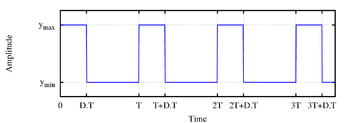
\includegraphics[width=5.35in,height=1.88in]{./media/image2.png}
	\end{Center}
\end{figure}


%%%%%%%%%%%%%%%%%%%% Figure/Image No: 2 Ends here %%%%%%%%%%%%%%%%%%%%

\par

\begin{justify}
La modulación por ancho de pulsos (también conocida como PWM, siglas en inglés de pulse-width modulation) de una señal o fuente de energía es una técnica en la que se modifica el ciclo de trabajo de una señal periódica (una senoidal o una cuadrada, por ejemplo), ya sea para transmitir información a través de un canal de comunicaciones o para controlar la cantidad de energía que se envía a una carga.
\end{justify}\par

\begin{justify}
El ciclo de trabajo de una señal periódica es el ancho relativo de su parte positiva en relación con el período. 
\end{justify}\par

\begin{justify}
Expresado matemáticamente:
\end{justify}\par

\begin{justify}
 \[ D=\frac{t}{T} \] 
\end{justify}\par

\begin{Center}
D es el ciclo de trabajo
\end{Center}\par

\begin{Center}
t es el tiempo en que la función es positiva (ancho del pulso)
\end{Center}\par

\begin{Center}
T es el período de la función
\end{Center}\par

\setlength{\parskip}{24.0pt}
{\fontsize{11pt}{13.2pt}\selectfont \textcolor[HTML]{474747}{La construcción típica de un circuito PWM se lleva a cabo mediante un comparador con dos entradas y una salida. Una de las entradas se conecta a un oscilador de onda dientes de sierra, mientras que la otra queda disponible para la señal moduladora. En la salida la frecuencia es generalmente igual a la de la señal dientes de sierra y el ciclo de trabajo está en función de la portadora.}\par}\par

{\fontsize{11pt}{13.2pt}\selectfont \textcolor[HTML]{474747}{La principal desventaja que presentan los circuitos PWM es la posibilidad de que haya interferencias generadas por radiofrecuencia. Éstas pueden minimizarse ubicando el controlador cerca de la carga y realizando un filtrado de la fuente de alimentación.}\par}\par


\vspace{\baselineskip}

\vspace{\baselineskip}

\vspace{\baselineskip}
\begin{Center}
\textbf{EJEMPLO DE GENERADOR DE SEÑAL MODULADA POR ANCHO DE PULSO}
\end{Center}\par

\begin{Center}
\textcolor[HTML]{656565}{Primero se procede a armar el esquemático del oscilador de relajación:}
\end{Center}\par



%%%%%%%%%%%%%%%%%%%% Figure/Image No: 3 starts here %%%%%%%%%%%%%%%%%%%%

\begin{figure}[H]
	\begin{Center}
		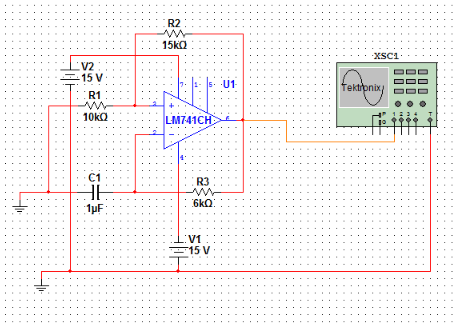
\includegraphics[width=5.81in,height=4.12in]{./media/image3.png}
	\end{Center}
\end{figure}


%%%%%%%%%%%%%%%%%%%% Figure/Image No: 3 Ends here %%%%%%%%%%%%%%%%%%%%
\newpage
\par

\setlength{\parskip}{15.0pt}
{\fontsize{11pt}{13.2pt}\selectfont \textcolor[HTML]{656565}{Para esto se supusieron los valores de R1 y R2 y C1, a partir de ahí se realizaron los siguientes cálculos para conocer el valor de R3:}\par}\par



%%%%%%%%%%%%%%%%%%%% Figure/Image No: 4 starts here %%%%%%%%%%%%%%%%%%%%

\begin{figure}[H]
	\begin{Center}
		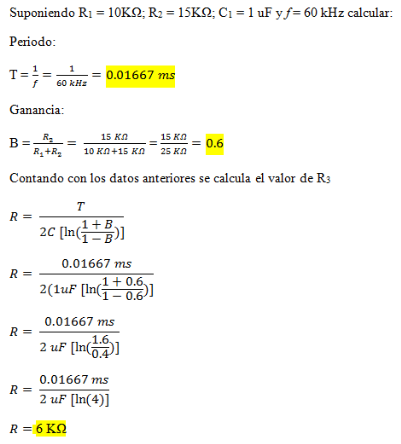
\includegraphics[width=4.1in,height=4.11in]{./media/image4.png}
	\end{Center}
\end{figure}


%%%%%%%%%%%%%%%%%%%% Figure/Image No: 4 Ends here %%%%%%%%%%%%%%%%%%%%

\par


\vspace{\baselineskip}
\begin{Center}
\textcolor[HTML]{656565}{Se conecta el osciloscopio y se mide voltaje pico-pico}
\end{Center}\par



%%%%%%%%%%%%%%%%%%%% Figure/Image No: 5 starts here %%%%%%%%%%%%%%%%%%%%

\begin{figure}[H]
	\begin{Center}
		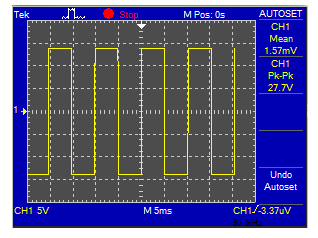
\includegraphics[width=3.09in,height=2.31in]{./media/image5.png}
	\end{Center}
\end{figure}


%%%%%%%%%%%%%%%%%%%% Figure/Image No: 5 Ends here %%%%%%%%%%%%%%%%%%%%

\par
\newpage
\begin{Center}
\textcolor[HTML]{656565}{y el tiempo que dura el ciclo:}
\end{Center}\par



%%%%%%%%%%%%%%%%%%%% Figure/Image No: 6 starts here %%%%%%%%%%%%%%%%%%%%

\begin{figure}[H]
	\begin{Center}
		
\includegraphics[width=2.93in,height=2.23in]{./media/image6.png}
	\end{Center}
\end{figure}


%%%%%%%%%%%%%%%%%%%% Figure/Image No: 6 Ends here %%%%%%%%%%%%%%%%%%%%

\par

\begin{Center}
\textcolor[HTML]{656565}{Se calcula el valor de R4 que será la que unirá ambos amplificadores operacionales y es por donde pasará la señal que posteriormente saldrá triangular:}
\end{Center}\par



%%%%%%%%%%%%%%%%%%%% Figure/Image No: 7 starts here %%%%%%%%%%%%%%%%%%%%

\begin{figure}[H]
	\begin{Center}
		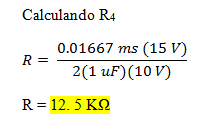
\includegraphics[width=2.05in,height=1.35in]{./media/image7.png}
	\end{Center}
\end{figure}


%%%%%%%%%%%%%%%%%%%% Figure/Image No: 7 Ends here %%%%%%%%%%%%%%%%%%%%

\par

\setlength{\parskip}{8.04pt}

\vspace{\baselineskip}
\begin{Center}
\textcolor[HTML]{656565}{Una vez que se conoce el valor de R4, se conecta el amplificador (comparador) que convierte la señal en triangular:}
\end{Center}\par



%%%%%%%%%%%%%%%%%%%% Figure/Image No: 8 starts here %%%%%%%%%%%%%%%%%%%%

\begin{figure}[H]
	\begin{Center}
		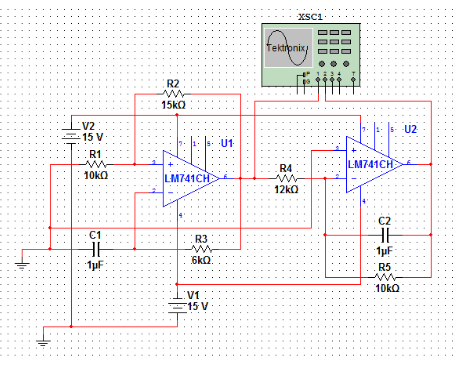
\includegraphics[width=4.3in,height=3.1in]{./media/image8.png}
	\end{Center}
\end{figure}


%%%%%%%%%%%%%%%%%%%% Figure/Image No: 8 Ends here %%%%%%%%%%%%%%%%%%%%

\par



%%%%%%%%%%%%%%%%%%%% Figure/Image No: 9 starts here %%%%%%%%%%%%%%%%%%%%

\begin{figure}[H]
	\begin{Center}
		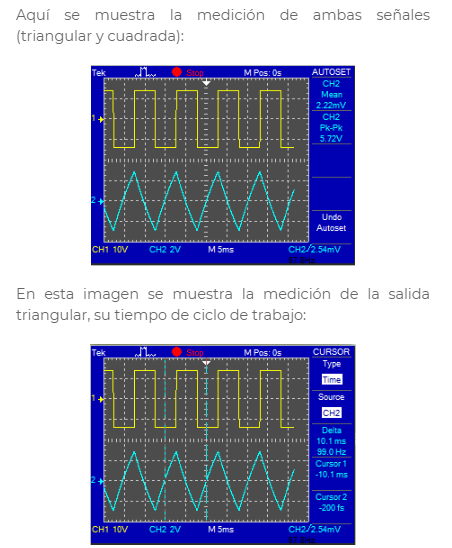
\includegraphics[width=4.29in,height=5.2in]{./media/image9.png}
	\end{Center}
\end{figure}


%%%%%%%%%%%%%%%%%%%% Figure/Image No: 9 Ends here %%%%%%%%%%%%%%%%%%%%

\par

\begin{Center}
\textcolor[HTML]{656565}{Se procede a armar el circuito en físico de la misma manera que en la simulación, primero el oscilador de relajación:}
\end{Center}\par



%%%%%%%%%%%%%%%%%%%% Figure/Image No: 10 starts here %%%%%%%%%%%%%%%%%%%%

\begin{figure}[H]
	\begin{Center}
		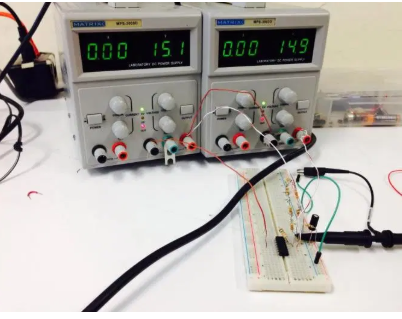
\includegraphics[width=4.19in,height=3.32in]{./media/image10.png}
	\end{Center}
\end{figure}


%%%%%%%%%%%%%%%%%%%% Figure/Image No: 10 Ends here %%%%%%%%%%%%%%%%%%%%

\par
\newpage
\setlength{\parskip}{15.0pt}
\begin{Center}
\textcolor[HTML]{656565}{Aquí se muestra la señal arrojada por este en el osciloscopio:}
\end{Center}\par



%%%%%%%%%%%%%%%%%%%% Figure/Image No: 11 starts here %%%%%%%%%%%%%%%%%%%%

\begin{figure}[H]
	\begin{Center}
		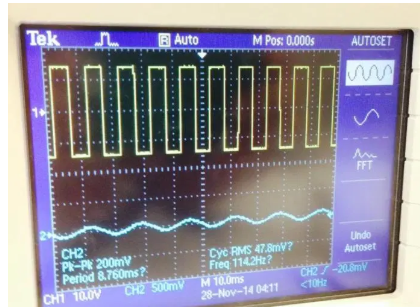
\includegraphics[width=3.03in,height=2.22in]{./media/image11.png}
	\end{Center}
\end{figure}


%%%%%%%%%%%%%%%%%%%% Figure/Image No: 11 Ends here %%%%%%%%%%%%%%%%%%%%

\href{https://carlosalbertosainz.files.wordpress.com/2014/12/pic1.jpg}{\\
}\par

\begin{Center}
\textcolor[HTML]{656565}{En esta imagen se observa su periodo, así como su voltaje pico-pico:}
\end{Center}\par



%%%%%%%%%%%%%%%%%%%% Figure/Image No: 12 starts here %%%%%%%%%%%%%%%%%%%%

\begin{figure}[H]
	\begin{Center}
		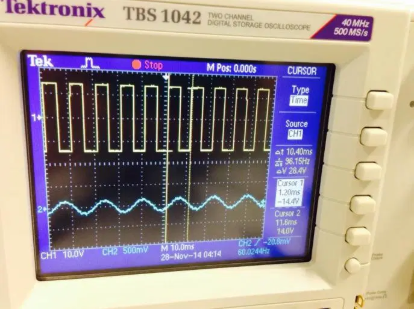
\includegraphics[width=2.79in,height=2.08in]{./media/image12.png}
	\end{Center}
\end{figure}


%%%%%%%%%%%%%%%%%%%% Figure/Image No: 12 Ends here %%%%%%%%%%%%%%%%%%%%

\par


\begin{Center}
\textcolor[HTML]{656565}{Ahora se une el integrador, los cálculos ya se habían realizado para la implementación:}
\end{Center}\par



%%%%%%%%%%%%%%%%%%%% Figure/Image No: 13 starts here %%%%%%%%%%%%%%%%%%%%

\begin{figure}[H]
	\begin{Center}
		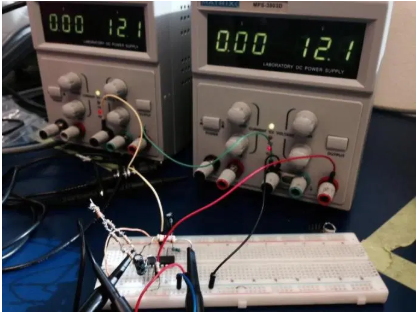
\includegraphics[width=4.0in,height=2.98in]{./media/image13.png}
	\end{Center}
\end{figure}


%%%%%%%%%%%%%%%%%%%% Figure/Image No: 13 Ends here %%%%%%%%%%%%%%%%%%%%

\par

\begin{Center}
\textcolor[HTML]{656565}{Se conectaron ambos amplificadores operacionales, en esta imagen se aprecia un LM que contiene cuatro amplificadores de manera interna:}
\end{Center}\par



%%%%%%%%%%%%%%%%%%%% Figure/Image No: 14 starts here %%%%%%%%%%%%%%%%%%%%

\begin{figure}[H]
	\begin{Center}
		
\includegraphics[width=4.41in,height=5.76in]{./media/image14.png}
	\end{Center}
\end{figure}


%%%%%%%%%%%%%%%%%%%% Figure/Image No: 14 Ends here %%%%%%%%%%%%%%%%%%%%

\par

\newpage
\begin{Center}
\textcolor[HTML]{656565}{Este circuito arroja la siguiente señal, en donde se aprecia que se mide la amplitud de la señal triangular:}
\end{Center}\par



%%%%%%%%%%%%%%%%%%%% Figure/Image No: 15 starts here %%%%%%%%%%%%%%%%%%%%

\begin{figure}[H]
	\begin{Center}
		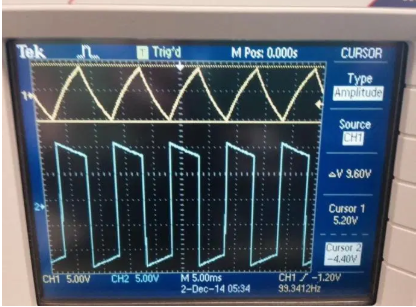
\includegraphics[width=4.33in,height=3.2in]{./media/image15.png}
	\end{Center}
\end{figure}


%%%%%%%%%%%%%%%%%%%% Figure/Image No: 15 Ends here %%%%%%%%%%%%%%%%%%%%

\par


\vspace{\baselineskip}
\begin{Center}
En esta otra imagen se muestra la misma señal, solamente que ahora se mide el periodo, pero además a la derecha se muestran otras mediciones que realiza el osciloscopio automáticamente:
\end{Center}\par



%%%%%%%%%%%%%%%%%%%% Figure/Image No: 16 starts here %%%%%%%%%%%%%%%%%%%%

\begin{figure}[H]
	\begin{Center}
		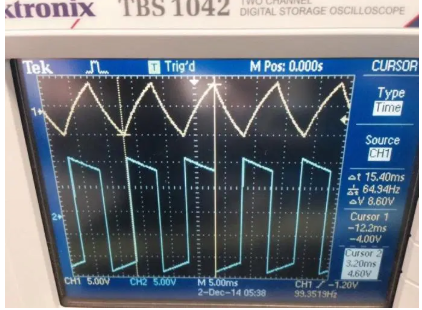
\includegraphics[width=4.4in,height=3.23in]{./media/image16.png}
	\end{Center}
\end{figure}


%%%%%%%%%%%%%%%%%%%% Figure/Image No: 16 Ends here %%%%%%%%%%%%%%%%%%%%

\par


\vspace{\baselineskip}

\vspace{\baselineskip}

\vspace{\baselineskip}

\vspace{\baselineskip}

\vspace{\baselineskip}

\vspace{\baselineskip}

\vspace{\baselineskip}

\vspace{\baselineskip}

\vspace{\baselineskip}

\vspace{\baselineskip}
\begin{Center}
\textcolor[HTML]{656565}{Estas son las mediciones de amplitud de la segunda señal:}
\end{Center}\par



%%%%%%%%%%%%%%%%%%%% Figure/Image No: 17 starts here %%%%%%%%%%%%%%%%%%%%

\begin{figure}[H]
	\begin{Center}
		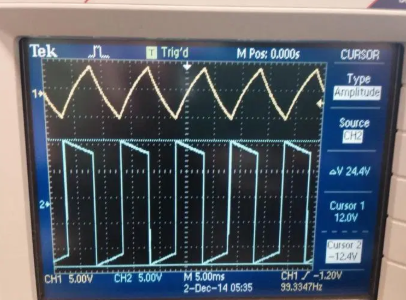
\includegraphics[width=4.23in,height=3.12in]{./media/image17.png}
	\end{Center}
\end{figure}


%%%%%%%%%%%%%%%%%%%% Figure/Image No: 17 Ends here %%%%%%%%%%%%%%%%%%%%

\par

\begin{Center}
\textcolor[HTML]{656565}{Aquí se midió el periodo de la señal del oscilador:} 
\end{Center}\par



%%%%%%%%%%%%%%%%%%%% Figure/Image No: 18 starts here %%%%%%%%%%%%%%%%%%%%

\begin{figure}[H]
	\begin{Center}
		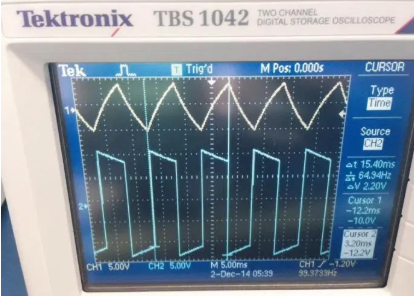
\includegraphics[width=4.31in,height=3.08in]{./media/image18.png}
	\end{Center}
\end{figure}


%%%%%%%%%%%%%%%%%%%% Figure/Image No: 18 Ends here %%%%%%%%%%%%%%%%%%%%

\par

\begin{Center}
\textcolor[HTML]{656565}{Después se procede a conectar un Potenciometro a la entrada inversora de otro amplificador operacional, a la entrada no inversora se conectará la salida triangular, esta se regula mediante el Potenciometro y se observa como varia el ancho de pulso de esta.}
\end{Center}\par

\setlength{\parskip}{8.04pt}
\textcolor[HTML]{33CCCC}{Conclusiones}\par

\textcolor[HTML]{656565}{Con esta práctica se comprendió como es que cada amplificador realiza una función en especifica al conectar de diferentes maneras las entradas inversoras y no inversoras de este. Funcionan de tal manera que al entrar una señal senoidal al oscilador de relajación sale cuadrada y al pasar al integrador se convierte en triangular.}\par

\textcolor[HTML]{656565}{Además, se observó como varia el ancho de pulso al introducir un voltaje de referencia y manipular la señal triangular que arroja el circuito comprendido por el oscilador de relajación y el integrador.}\par


\vspace{\baselineskip}

\printbibliography
\end{document}